\documentclass{standalone}
\usepackage{preset}
\begin{document}
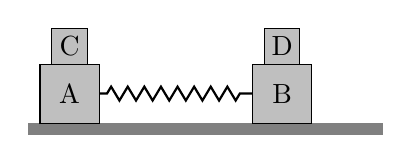
\begin{tikzpicture}[x=15mm,y=15mm]
	\tikzstyle{spring}=[thick,decorate,decoration={zigzag,pre length=0.1cm,post length=0.1cm,segment length=6}]
	\draw(0,0)--(3,0);
	\draw[draw=none,fill=gray](0,0)rectangle(3,-.1);
	\draw[spring](.6,.25)--(1.9,.25);
	\tikzset{every path/.style={fill=lightgray}}
	\draw(.1,0)rectangle node{A}+(.5,.5);
	\draw(.2,.5)rectangle node{C}+(.3,.3);
	\draw(1.9,0)rectangle node{B}+(.5,.5);
	\draw(2,.5)rectangle node{D}+(.3,.3);
\end{tikzpicture}
\end{document}
